\section{Systembeskrivelse}
For at gøre det muligt, at anvende det samme system på 4. Semester skal arbejdsområdet kunne benyttes sammen med et USB-baserede trådløst udviklingsværktøj eZ430-RF2500 fra Texas Instruments. Det er derfor nødvendigt, at designet stemmer overens med udviklingsværktøjet for at kunne sende og modtage data til og fra computeren. Udviklingsværktøjet indeholder hardware og software som evaluerer mikrokontrolleren MSP430F2274. For at systemet kan anvendes med udviklingsværktøjet skal outputsignalet være 3V, eftersom mikrokontrolleren opererer med spændingsforsyning mellem 1,8 V og 3,6 V.  

\subsection{Formål og anvendelse}
Ud fra problemanalysen fremgår det, at apopleksipatienter ofte er ældre over 65 år og en af de hyppigste følger de oplever er balanceproblemer. For apopleksipatienter er behovet for at være selvstændige og uafhængige af hjælp vigtigt.\ref{til problemafgrænsningen eller problemanalysen}  
Derfor er et system som opfanger, hvis patienten er ude af balance at foretrække, det skal kunne anvendes selvstændigt i hjemmet dvs. uden hjælp fra nogen form for plejepersonale. Dette vil sige, at systemet skal implementeres i fase 4 \ref{rehabilitering faseafsnittet}. Dette kræver at selve systemet er brugervenligt dvs. at det skal være let at påsætte, ikke veje for meget samt signalerne skal være let forståelig. Dette kræves, da størstedelen af apopleksipatienter som nævnt er ældre og kan opleve kognitive problemer \ref{...}. Dette giver også begrænsninger i forhold til feedback, da både hørelsen, synet eller kroppens følelser kan være svækket i forbindelse med, at patienterne bliver ældre\ref{findnykilde}. Derudover skal systemet kunne give et analogt og digitalt output, som er muligt at behandle.


\subsection{Beskrivelse af test}
Patienten skal være stående og have fødderne på linje, dette fremgår som udgangsposition\fxnote{måske et billede vi tager som vil illustrere dette}. Netop denne position anvendes for at udfordre patienten ved at fordele kropsvægten anderledes i forhold til den normale kropsstilling.\ref{balanceafsnittet} Patienten påsætter systemet og udfører herefter en prøvetest for at kende til den feedback der gives. Prøvetesten går ud på at hælde langsomt fra side til side. Hvis patienten hælder lidt, hvor det er usikkert, vil en lampe lyse gult og patienten vil kunne mærke vibration. Hvis patienten ikke retter op og ender i en riskozone vil en anden lampe lyse rødt. Vibrationen vil stige i takt med at lyset ændre sig fra gult til rødt. Selve øvelsen udføres herefter ved at holde balancen i udgangspositionen, herefter lukkes øjnene for at udelukke en af sanserne, hvilket gør det svære for patienten at opretholde balancen \ref{balanceafsnittet}. Selve forsøget gentages 5 gange af 3 minutter\fxnote{ved ikke hvor langt tid og hvor mange gange}.

\subsection{Analogt output}
Det analoge output skal kunne henvende sig til patienten, dette sker ved lysdioder og vibration. Lysdioderne skal lyse gult ved 'usikkerhed' og slukke hvis patienten enten er rettet op igen eller bevæger sig ud i riskozonen, hvorefter en nye diode skal lyse rødt. Vibrationerne igangsættes ved 'usikkerhed' og skal stoppe hvis patienten retter sig op eller stige i styrke, hvis patienten kommer i risikozonen. 

\subsection{Digitalt output}
Det digitale skal kunne anvendes af sundhedspersonale til at vurdere om patienten gør fremskridt, dette indebærer at informationerne for patienten kan gemmes og sammenlignes på en computer. 


\subsection{Systemets opbygning}
Systemets opbygning fremgår af \figref{krav_blok}. Når signalet er opsamlet ved et accelerometer, sendes signalet osv....

\begin{figure}[H]
	\centering
	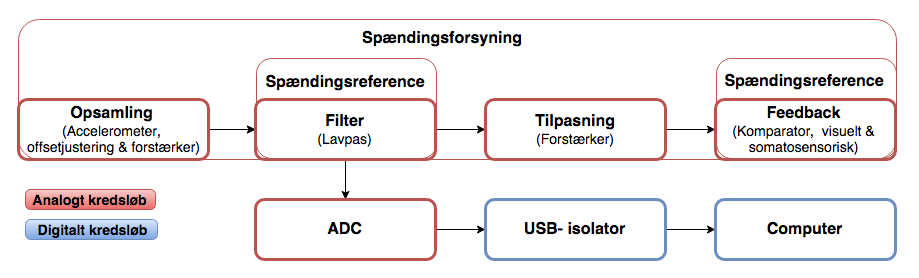
\includegraphics[scale=0.8]{figures/cProblemløsning/blokdiagram.png}
	\caption{Figuren viser de blokke/elementer som systemet skal indeholde}
	\label{krav_blok}
\end{figure}

\subsection{Kravspecifikationer}
\begin{itemize}
\item Systemet skal anvendes visuel og sensorisk feedback 
\item Systemet skal være non-invasiv - dvs. systemet må ikke påføre patienten smerte eller varig skade
\item Systemet skal være brugervenlig
\item Systemet skal forsynes med spænding fra et batteri
\end{itemize}

%\subsubsection{Accelerometer}
%Accelerometeret skal detektere patientens kropshældning.

%\subsubsection{Filter}
%Når der anvendes et filter, skal det dæmpe uønskede frekvenser. Dvs. frekvenser der lavere eller højere ift. det signal fra accelerometeret, som man vil analysere på. Der skal udføres et pilotforsøg for at finde frem til det korrekte filter og valg af knækfrekvens. 

%\subsubsection{Signalerende lys}
%Når patienten er ude af balance skal en rød diode lyse, som signalering ift. patientens hældning. Der skal vha. et pilotforsøg detekteres, hvornår dioden skal lyse. Skal der evt. være 2 dioder, hvor den ene er et "advarende" signal og nr. to er "fare". 

%\subsubsection{Alarm/vibrationen}
%Alarmen/vibrationen skal anvendes i perioden, hvor patienten er ude af balance og stoppe igen, når der igen er oprettet balance. 
%(eller fungere som en alarm til dioderne - så når en diode lyser, skal alarmen gå)

\subsubsection{ADC}
Der anvendes en ADC i systemet, for at konvertere det analoge signal til digitalt. Det næste skridt er konverteringen til PC og det er derfor essentielt at have en ADC, der konverterer analogt signal til binære tal, som digitale systemet anvender. 
{Her skal vi have valgt en samplingsfrekvens)

\subsubsection{USB-isolater}
USB-isolatoren sikre patientens sikkerhed. Her skal input- og outputspænding være ens.  

\subsubsection{Til PC}
Fremvisning af graf, så patienten og plejepersonale kan følge rehabiliteringens udvikling. 

% Inspiration især fra: Brug af Biofeedback til Rehabilitering af Apopleksipatienter 